\documentclass[11pt,a4paper]{article}
\usepackage[utf8]{inputenc}
\usepackage[T1]{fontenc}
\usepackage[spanish,es-noshorthands]{babel}
\usepackage{lmodern}
\usepackage[margin=2.2cm,headheight=1.6cm,includehead]{geometry}
\usepackage{amsmath,amssymb}
\usepackage{graphicx}
\usepackage{booktabs,tabularx,array}
\usepackage{fancyhdr,lastpage}
\usepackage[locale=DE,group-separator={.},group-minimum-digits=4,group-digits=integer]{siunitx}
\usepackage{xcolor}
\usepackage[hidelinks]{hyperref}

% Generado por scripts/exportar_datos.py -- no editar a mano
% Planilla: Rullo_PSV_estatico_fatiga.xlsx
\newcommand{\vAg}{\num{29800}}
\newcommand{\vAmD}{\num{15330}}
\newcommand{\vAmI}{\num{706.9}}
\newcommand{\vArea}{\num{4075}}
\newcommand{\vB}{\num{1110}}
\newcommand{\vD}{\num{139.7}}
\newcommand{\vDextmD}{\num{30}}
\newcommand{\vDextmI}{\num{30}}
\newcommand{\vDintmD}{\num{0}}
\newcommand{\vDintmI}{\num{0}}
\newcommand{\vDp}{\num{200}}
\newcommand{\vE}{\num{207000}}
\newcommand{\vF}{\num{12770}}
\newcommand{\vFp}{\num{0}}
\newcommand{\vFpy}{\num{0}}
\newcommand{\vFpz}{\num{0}}
\newcommand{\vFu}{\num{34.67}}
\newcommand{\vG}{\num{40}}
\newcommand{\vI}{\num{8619000}}
\newcommand{\vJ}{\num{17240000}}
\newcommand{\vKp}{\num{1.5}}
\newcommand{\vL}{\num{1230}}
\newcommand{\vLg}{\num{1130}}
\newcommand{\vLmD}{\num{20}}
\newcommand{\vLmI}{\num{80}}
\newcommand{\vLp}{\num{1429}}
\newcommand{\vLt}{\num{337.9}}
\newcommand{\vLtin}{\num{0}}
\newcommand{\vLtubo}{\num{1130}}
\newcommand{\vMeje}{\num{38.99}}
\newcommand{\vMgoma}{\num{43.77}}
\newcommand{\vMmax}{\num{2150000}}
\newcommand{\vMp}{\num{0}}
\newcommand{\vMrot}{\num{82.77}}
\newcommand{\vP}{\num{4}}
\newcommand{\vRdos}{\num{6815}}
\newcommand{\vRdosy}{\num{6800}}
\newcommand{\vRdosz}{\num{449.2}}
\newcommand{\vRuno}{\num{5982}}
\newcommand{\vRunoy}{\num{5970}}
\newcommand{\vRunoz}{\num{390}}
\newcommand{\vSe}{\num{107.1}}
\newcommand{\vSemD}{\num{123.4}}
\newcommand{\vSemI}{\num{153}}
\newcommand{\vSep}{\num{190}}
\newcommand{\vSu}{\num{380}}
\newcommand{\vSuMD}{\num{380}}
\newcommand{\vSuMI}{\num{380}}
\newcommand{\vSy}{\num{210}}
\newcommand{\vSyMD}{\num{210}}
\newcommand{\vSyMI}{\num{210}}
\newcommand{\vTb}{\num{172.6}}
\newcommand{\vTcero}{\num{382000}}
\newcommand{\vTtot}{\num{6385}}
\newcommand{\vUper}{\num{316100}}
\newcommand{\vUperD}{\num{169200}}
\newcommand{\vUperI}{\num{146900}}
\newcommand{\vVa}{\num{1092}}
\newcommand{\vVc}{\num{5.95}}
\newcommand{\vWz}{\num{27.22}}
\newcommand{\vainicio}{\num{100}}
\newcommand{\vbfin}{\num{20}}
\newcommand{\vbw}{\num{30}}
\newcommand{\vchk}{\num{0}}
\newcommand{\vcp}{\num{80}}
\newcommand{\vcsb}{\num{0.847}}
\newcommand{\vcsg}{\num{0.7708}}
\newcommand{\vdint}{\num{119.7}}
\newcommand{\veg}{\num{50}}
\newcommand{\velec}{E70xx}
\newcommand{\veper}{\num{3820}}
\newcommand{\veu}{\num{0}}
\newcommand{\vexc}{\num{3.82}}
\newcommand{\vfC}{\num{1}}
\newcommand{\vfS}{\num{0.8108}}
\newcommand{\vfT}{\num{0.6953}}
\newcommand{\vfl}{\num{0.2634}}
\newcommand{\vflb}{\num{1.161}}
\newcommand{\vflg}{\num{1.057}}
\newcommand{\vfr}{\num{60}}
\newcommand{\vfuno}{\num{1}}
\newcommand{\vgar}{\num{0}}
\newcommand{\vkKfdos}{\num{2.197}}
\newcommand{\vkKfsdos}{\num{1.913}}
\newcommand{\vkKfstres}{\num{1.913}}
\newcommand{\vkKfsuno}{\num{1.913}}
\newcommand{\vkKftres}{\num{2.197}}
\newcommand{\vkKfuno}{\num{2.197}}
\newcommand{\vkKtdos}{\num{1}}
\newcommand{\vkKtsdos}{\num{1}}
\newcommand{\vkKtstres}{\num{2.2}}
\newcommand{\vkKtsuno}{\num{2.2}}
\newcommand{\vkKttres}{\num{2.7}}
\newcommand{\vkKtuno}{\num{2.7}}
\newcommand{\vkcsdos}{\num{2.775}}
\newcommand{\vkcstres}{\num{9.627}}
\newcommand{\vkcsuno}{\num{0.7708}}
\newcommand{\vkfldos}{\num{5.481}}
\newcommand{\vkfltres}{\num{17.14}}
\newcommand{\vkfluno}{\num{1.057}}
\newcommand{\vkondos}{1}
\newcommand{\vkontres}{1}
\newcommand{\vkonuno}{1}
\newcommand{\vkrdos}{\num{2}}
\newcommand{\vkrtres}{\num{2}}
\newcommand{\vkruno}{\num{2}}
\newcommand{\vksados}{\num{38.25}}
\newcommand{\vksatres}{\num{10.42}}
\newcommand{\vksauno}{\num{198.4}}
\newcommand{\vksmdos}{\num{1.208}}
\newcommand{\vksmtres}{\num{2.512}}
\newcommand{\vksmuno}{\num{0.2531}}
\newcommand{\vkvidados}{Vida infinita}
\newcommand{\vkvidatres}{Vida infinita}
\newcommand{\vkvidauno}{\num{106800}}
\newcommand{\vkxdos}{\num{600}}
\newcommand{\vkxtres}{\num{1140}}
\newcommand{\vkxuno}{\num{40}}
\newcommand{\vlado}{0}
\newcommand{\vmb}{\num{0.15}}
\newcommand{\vmlin}{\num{0.105}}
\newcommand{\vmu}{\num{70.72}}
\newcommand{\vn}{\num{100}}
\newcommand{\vnb}{\num{37}}
\newcommand{\vnc}{\num{9894}}
\newcommand{\vomega}{\num{10.47}}
\newcommand{\vpm}{1}
\newcommand{\vpp}{1}
\newcommand{\vqy}{\num{11.5}}
\newcommand{\vqz}{\num{0.02453}}
\newcommand{\vrFu}{\num{0.002715}}
\newcommand{\vrf}{\num{0}}
\newcommand{\vrho}{\num{7.85e-06}}
\newcommand{\vrhog}{\num{1.3e-06}}
\newcommand{\vrnc}{\num{0.01011}}
\newcommand{\vskfder}{\num{1.2}}
\newcommand{\vskfizq}{\num{1.5}}
\newcommand{\vsseder}{\num{97.41}}
\newcommand{\vsseizq}{\num{97.41}}
\newcommand{\vscsder}{\num{12.79}}
\newcommand{\vscsizq}{\num{4.668}}
\newcommand{\vsflder}{\num{21.83}}
\newcommand{\vsflizq}{\num{10.05}}
\newcommand{\vsgder}{\num{10}}
\newcommand{\vsgizq}{\num{5.656}}
\newcommand{\vsmax}{\num{180.4}}
\newcommand{\vsobre}{Con sobremonta}
\newcommand{\vsrev}{\num{198.5}}
\newcommand{\vssader}{\num{1.325}}
\newcommand{\vssaizq}{\num{4.654}}
\newcommand{\vssmder}{\num{2.681}}
\newcommand{\vssmizq}{\num{0.01051}}
\newcommand{\vssuder}{\num{380}}
\newcommand{\vssuizq}{\num{380}}
\newcommand{\vstipoder}{A tope}
\newcommand{\vstipoizq}{Filete}
\newcommand{\vsvidader}{Vida infinita}
\newcommand{\vsvidaizq}{Vida infinita}
\newcommand{\vswfl}{1}
\newcommand{\vswp}{0}
\newcommand{\vsxder}{\num{1210}}
\newcommand{\vsxizq}{\num{80}}
\newcommand{\vt}{\num{10}}
\newcommand{\vterm}{Laminado en caliente}
\newcommand{\vtermMD}{Maquinado o estirado en frío}
\newcommand{\vtermMI}{Maquinado o estirado en frío}
\newcommand{\vthp}{\num{0}}
\newcommand{\vtsiga}{\num{180.4}}
\newcommand{\vtsigm}{\num{0.4889}}
\newcommand{\vttauaB}{\num{11.28}}
\newcommand{\vttaum}{\num{0}}
\newcommand{\vttaumB}{\num{0.02845}}
\newcommand{\vtvma}{\num{180.4}}
\newcommand{\vtvmaB}{\num{19.54}}
\newcommand{\vtvmm}{\num{0.4889}}
\newcommand{\vtvmmB}{\num{0.04927}}
\newcommand{\vtvmmax}{\num{180.9}}
\newcommand{\vtxcrit}{\num{79.95}}
\newcommand{\vub}{1}
\newcommand{\vw}{\num{0.3138}}
\newcommand{\vwf}{\num{8}}
\newcommand{\vwg}{\num{0.38}}
\newcommand{\vwmD}{\num{1.18}}
\newcommand{\vwmI}{\num{0.05443}}
\newcommand{\vwu}{\num{0.02819}}
\newcommand{\vxG}{\num{658.5}}
\newcommand{\vxM}{\num{621.1}}
\newcommand{\vxcsb}{\num{79.95}}
\newcommand{\vxfl}{\num{522.8}}
\newcommand{\vxgcero}{\num{80}}
\newcommand{\vxsD}{\num{1210}}
\newcommand{\vxsI}{\num{80}}
\newcommand{\vxtope}{\num{0}}
\newcommand{\vxtp}{\num{1210}}
\newcommand{\vFilasConc}{1 & \vkxuno & \vkKtuno & \vkKtsuno & \vkruno & \vkKfuno & \vksauno & \vksmuno & \vkcsuno & \vkfluno \\ 2 & \vkxdos & \vkKtdos & \vkKtsdos & \vkrdos & \vkKfdos & \vksados & \vksmdos & \vkcsdos & \vkfldos \\ 3 & \vkxtres & \vkKttres & \vkKtstres & \vkrtres & \vkKftres & \vksatres & \vksmtres & \vkcstres & \vkfltres \\}
\newcommand{\vgeomok}{1}
\newcommand{\vFechaDatos}{16/11/2026}
\newcommand{\vArchivo}{Rullo\_PSV\_estatico\_fatiga.xlsx}


% ---------------------------------------------------------------- encabezado
\newcommand{\titulo}{Memoria de cálculo -- Rullo delantero torno PSV}
\pagestyle{fancy}
\fancyhf{}
\fancyhead[L]{\IfFileExists{figuras/logo_dayco.png}{\includegraphics[height=1.1cm]{figuras/logo_dayco.png}}{\textsf{DAYCO}}}
\fancyhead[R]{\small\titulo}
\fancyfoot[R]{\small Página \thepage\ de \pageref{LastPage}}
\fancyfoot[L]{\small Datos: \vArchivo\ (\vFechaDatos)}
\renewcommand{\headrulewidth}{0.4pt}

\newcommand{\supu}{\textsuperscript{*}}   % supuesto a validar
\setlength{\parindent}{0pt}
\setlength{\parskip}{4pt}

\begin{document}

\begin{center}
{\Large\bfseries \titulo}\\[2mm]
Verificación estática y a fatiga\\
\small Fuente de cálculo: Compendio de Cálculo Estructural II, FCEFyN--UNC 2024, cap.~14
\end{center}

% =================================================================
\section{Objeto}
Verificar a fluencia y a fatiga el rullo delantero (motriz) del torno PSV, que trabaja entre dos
rodamientos, con los datos cargados en la planilla \texttt{\vArchivo}. Los valores marcados
con \supu\ corresponden a supuestos a validar (sección~\ref{sec:sup}).

% =================================================================
\section{Modelo}
Viga simplemente apoyada en los centros de los rodamientos. Ejes: $x$ a lo largo del rullo desde el
apoyo izquierdo, $y$ en la dirección de la tensión del manchón y $z$ en la dirección de la gravedad.
Cada plano se resuelve por separado y se combinan $M=\sqrt{M_y^2+M_z^2}$ y $V=\sqrt{V_y^2+V_z^2}$
(sección circular). El eje gira y las cargas tienen dirección fija, por lo que la flexión es
completamente alternante (un ciclo por vuelta).

\begin{center}
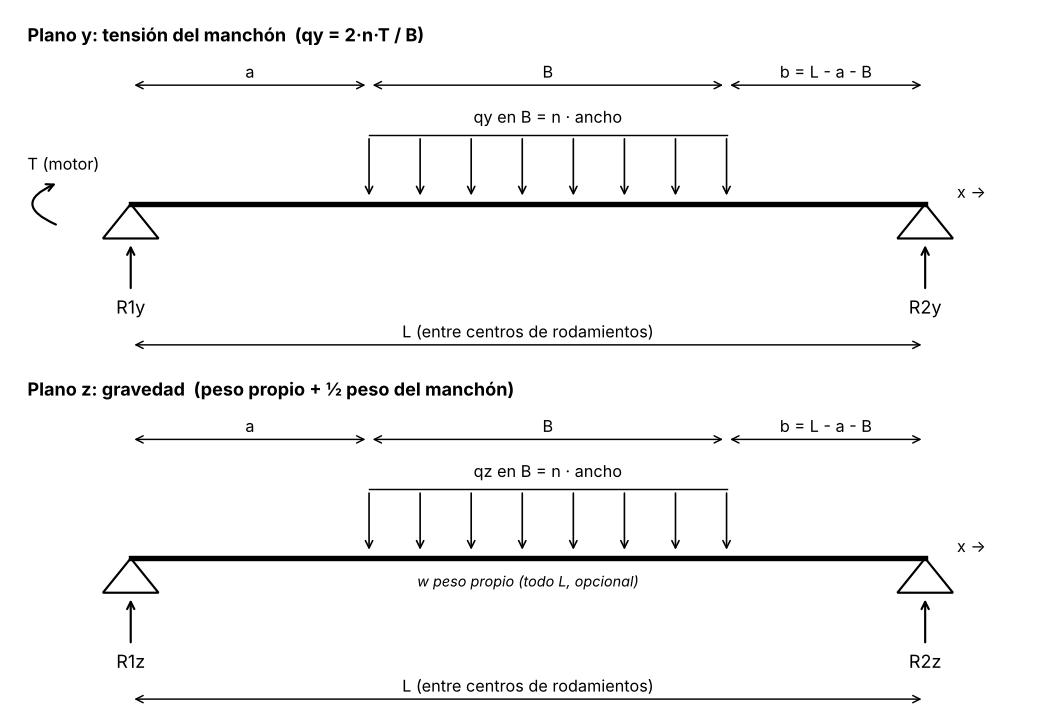
\includegraphics[width=0.85\textwidth]{figuras/dcl.png}
\end{center}

% =================================================================
\section{Datos}
\begin{center}
\begin{tabular}{lrl@{\hspace{1.2cm}}lrl}
\toprule
\multicolumn{3}{c}{Tubo y material} & \multicolumn{3}{c}{Manchón} \\
\midrule
$D$ exterior     & \vD   & mm  & Cantidad de correas $n$ & \vnb & -- \\
Espesor $t$      & \vt   & mm  & Ancho por correa        & \vbw & mm \\
$L$ entre apoyos & \vL   & mm  & Masa por correa         & \vmb & kg \\
$S_u$            & \vSu  & MPa & Desarrollo              & \vLp & mm \\
$S_y$            & \vSy  & MPa & Frecuencia medida $f$   & \vfr & Hz \\
$E$              & \vE   & MPa & Inicio $a$              & \vainicio & mm \\
Engomado $e$\supu & \veg  & mm  & & & \\
\midrule
\multicolumn{3}{c}{Accionamiento} & \multicolumn{3}{c}{Superficie} \\
\midrule
Potencia $P$ & \vP & kW  & \multicolumn{3}{l}{\vterm} \\
Velocidad $n$ & \vn & rpm & & & \\
\bottomrule
\end{tabular}
\end{center}

Propiedades de la sección de acero (la goma no aporta rigidez\supu): $d=\vdint$~mm, $A=\vArea$~mm$^2$, $I=\vI$~mm$^4$, $J=\vJ$~mm$^4$.

% =================================================================
\section{Cargas}
\textbf{Tensión del manchón (plano $y$)\supu.} A partir de la frecuencia del ramal libre (cuerda vibrante):
\[
m=\frac{\text{masa}}{\text{desarrollo}}=\vmlin~\text{kg/m},\qquad
L_t=\vLt~\text{mm},\qquad
T=4\,m\,L_t^2\,f^2=\vTb~\text{N por correa}
\]
Con ramales paralelos la fuerza sobre el rullo es $F=2\,n\,T=\vF$~N, repartida en el ancho del
manchón $B=n\cdot\text{ancho}=\vB$~mm: $q_y=F/B=\vqy$~N/mm, entre $x=a$ y $x=a+B$ ($b=\vbfin$~mm).

\textbf{Gravedad (plano $z$).} Peso propio de tubo y engomado $w=\vw$~N/mm en todo $L$ y mitad del peso del
manchón\supu\ $q_z=\vqz$~N/mm en $B$.

\textbf{Torque.} $T=P/\omega=\vTcero$~N$\cdot$mm, constante; entra por un extremo y lo toman las
correas de forma pareja en $B$\supu.

\textbf{Reacciones} (equilibrio por plano):
\begin{center}
\begin{tabular}{lrrr}
\toprule
 & Plano $y$ [N] & Plano $z$ [N] & Resultante [N] \\
\midrule
Rodamiento izquierdo & \vRunoy & \vRunoz & \vRuno \\
Rodamiento derecho   & \vRdosy & \vRdosz & \vRdos \\
\bottomrule
\end{tabular}
\end{center}

% =================================================================
\section{Esfuerzos, tensiones y flecha}
\begin{center}
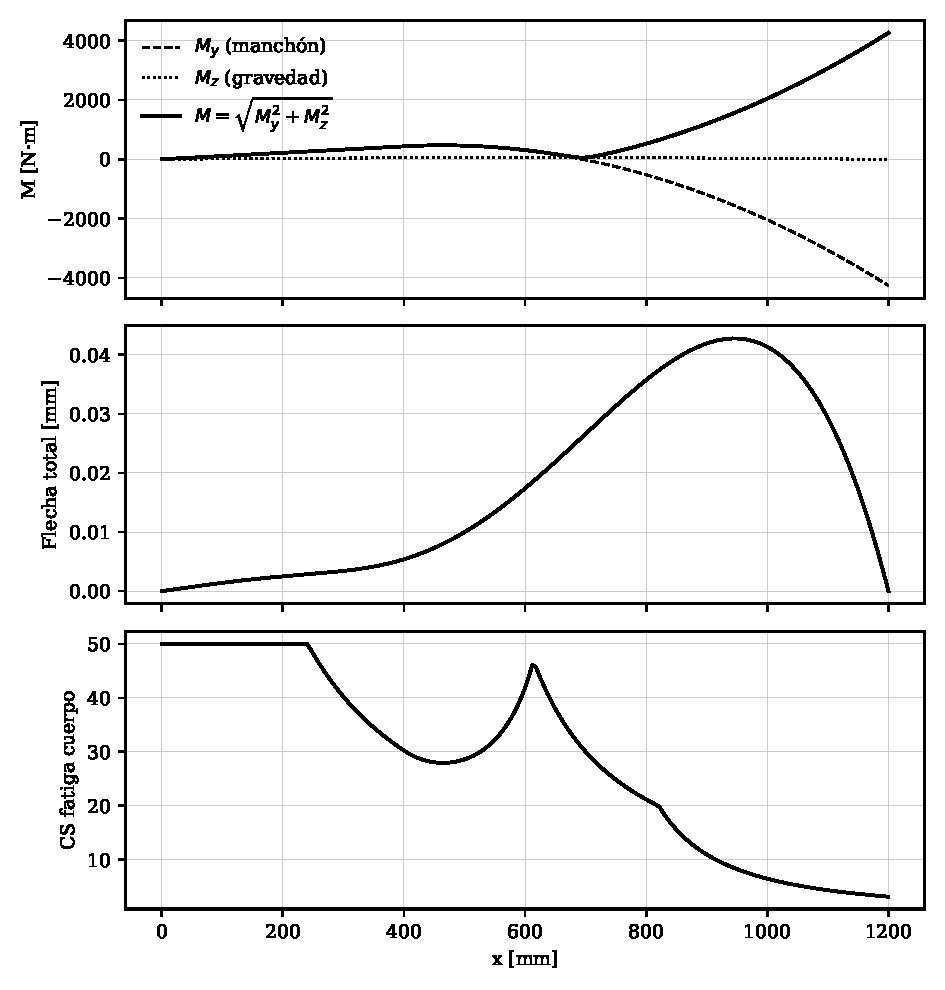
\includegraphics[width=0.85\textwidth]{figuras/diagramas.pdf}
\end{center}
Momento máximo $M=\vMmax$~N$\cdot$mm en $x=\vxM$~mm; $\sigma_0=M\,c/I=\vsmax$~MPa.
Flecha máxima \vfl~mm en $x=\vxfl$~mm (doble integración numérica de $M_y/EI$ y $M_z/EI$).

% =================================================================
\section{Fatiga}
\textbf{Resistencia de la pieza}, ec.~(20):
$S_e=f_T\,f_C\,f_S\,f_1\,S_e'=\vfT\cdot\vfC\cdot\vfS\cdot\vfuno\cdot\vSep=\vSe$~MPa,
con $S_e'=0{,}5\,S_u\le 690$~MPa (17), $f_T$ (21) con $D$ exterior\supu, $f_C=1$ por carga combinada (24) y
$f_S=a\,S_u^{\,b}$ (25)--(26).

\textbf{Procedimiento} (sección 7.1): tensor medio y tensor alternante; $K_f$ solo sobre la
componente alternante (Tabla~14, material dúctil); Von Mises de cada tensor (72); Goodman (44)-b;
fluencia por separado con el tensor máximo (77).

\textbf{Sección crítica del cuerpo} ($x=\vtxcrit$~mm, $K_f=1$, punto en la fibra extrema;
$x$ axial, $y$ radial, $z$ tangente, MPa):
\[
\sigma_m=\begin{bmatrix}0&0&\vttaum\\0&0&0\\\vttaum&0&0\end{bmatrix}
\qquad
\sigma_a=\begin{bmatrix}\vtsiga&0&0\\0&0&0\\0&0&0\end{bmatrix}
\qquad
\sigma_{\max}=\sigma_m+\sigma_a
\]
\[
\sigma'_m=\vtvmm,\qquad \sigma'_a=\vtvma,\qquad \sigma'_{\max}=\vtvmmax~\text{MPa}
\]
\[
CS_{\text{fatiga}}=\frac{1}{\sigma'_m/S_u+\sigma'_a/S_e}=\vcsb
\qquad\qquad
CS_{\text{fluencia}}=\frac{S_y}{\sigma'_{\max}}=\vflb
\]

\textbf{Diagrama S-N de la pieza} (ecs.~29--32): recta entre $(10^3;\,0{,}9S_u)$ y $(10^6;\,S_e)$,
horizontal después de $10^6$. La línea de trazos es la tensión alternante equivalente de la sección más
solicitada, $\sigma_a/(1-\sigma'_m/S_u)=\vsrev$~MPa (48-b).
\begin{center}
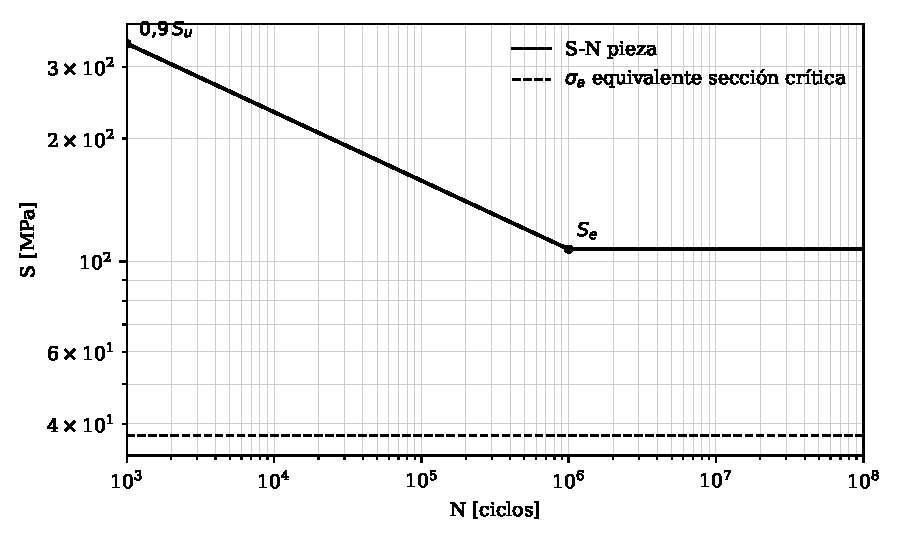
\includegraphics[width=0.75\textwidth]{figuras/diagrama_sn.pdf}
\end{center}

\textbf{Secciones con concentrador.} $K_f=1+q(K_t-1)$ (6), $q$ según Neuber (9)--(10)\supu.
$K_t$ y $K_{ts}$ del Anexo~2.
\begin{center}
\begin{tabular}{lccccccccl}
\toprule
Sección & $x$ [mm] & $K_t$ & $K_{ts}$ & $r$ [mm] & $K_f$ & $\sigma'_a$ & $\sigma'_m$ & $CS_{\text{fat}}$ & $CS_{\text{fl}}$ \\
\midrule
\vFilasConc
\bottomrule
\end{tabular}
\end{center}
Kf en la verificación a fluencia: \ifnum\vswfl=1 aplicado\else no aplicado\fi\supu.

% =================================================================
\section{Resultados}
\begin{center}
\begin{tabular}{lr}
\toprule
CS fatiga mínimo (Goodman) & \vcsg \\
CS fluencia mínimo         & \vflg \\
Flecha máxima [mm]         & \vfl \\
\bottomrule
\end{tabular}
\end{center}
Un $CS_{\text{fatiga}}<1$ indica vida limitada (ecs.~48-b y 32); el valor admisible queda a criterio del diseñador\supu.

% =================================================================
\section{Verificaciones complementarias\supu}
Fuera del compendio.
\begin{itemize}\setlength\itemsep{1pt}
\item Primera velocidad crítica de flexión (viga uniforme simplemente apoyada, sin masa del manchón):
$n_c=\frac{30}{\pi}\left(\frac{\pi}{L}\right)^2\sqrt{EI/\mu}=\vnc$~rpm; $n/n_c=\vrnc$.
\item Desbalanceo residual con grado $G=\vG$~mm/s (ISO 21940-11, rotor rígido): $F_u=M\,G\,\omega=\vFu$~N,
$F_u/F=\vrFu$. Gira con el eje, por lo que en el material produce tensión media, no alternante.
\end{itemize}

\noindent\textbf{Masa que gira y desbalance admisible.} El eje es el tubo entre soldaduras
($L_{\text{tubo}}=\vLtubo$~mm) más los dos muñones hacia afuera; el engomado se cuenta aparte.
\begin{center}
\begin{tabular}{llr}
\toprule
Masa del eje & $M_{\text{eje}}=\rho\,(A\,L_{\text{tubo}}+A_{mI}L_{mI}+A_{mD}L_{mD})$ & \vMeje~kg \\
Masa del engomado & $M_{\text{goma}}=\rho_g\,A_g\,L_g$ & \vMgoma~kg \\
Masa que gira & $M=M_{\text{eje}}+M_{\text{goma}}$ & \vMrot~kg \\
Centro de masa & $x_G=\sum m_i x_i/M$ & \vxG~mm \\
Excentricidad admisible & $e_{per}=1000\,G/\omega$ & \veper~g·mm/kg \\
Desbalance admisible & $U_{per}=e_{per}\,M$ & \vUper~g·mm \\
Apoyo izquierdo\supu & $U_{per}\,(L-x_G)/L$ & \vUperI~g·mm \\
Apoyo derecho\supu & $U_{per}\,x_G/L$ & \vUperD~g·mm \\
\bottomrule
\end{tabular}
\end{center}

% =================================================================
\section{Supuestos y limitaciones}\label{sec:sup}
\begin{itemize}\setlength\itemsep{1pt}
\item[\supu] Tensión por correa $T=4\,m\,L_t^2\,f^2$ (cuerda vibrante): no figura en el compendio.
\item[\supu] $L_t=(\text{desarrollo}-\pi D)/2$ si no se mide: ramales paralelos y rullos de igual diámetro.
\item[\supu] Mitad del peso del manchón sobre cada rullo.
\item[\supu] Engomado: solo peso y diámetro de apoyo del manchón ($D+2e$); densidad típica de caucho si no se carga el dato real.
\item[\supu] Torque constante, tomado por las correas de forma pareja en $B$.
\item[\supu] Desbalance: un solo grado $G$ para todo el rotor (eje + engomado). Reparto de $U_{per}$ en los apoyos por palanca respecto del centro de masa: verificar contra ISO 21940-11.
\item[\supu] La velocidad crítica y el peso propio toman tubo + goma en todo $L$, sin muñones ni el largo real del engomado.
\item[\supu] $f_T$ con el diámetro exterior del tubo; $K_{fs}$ aplicado al corte transversal en el eje neutro.
\item[\supu] Coeficientes de Neuber leídos del texto del compendio: verificar contra el impreso.
\item[\supu] $K_f$ en fluencia: ec.~(3) frente a ec.~(77), pendiente de definir.
\item No incluye uniones soldadas ni atornilladas, cargas de la cuchilla ni efectos dinámicos.
\item Fatiga de ciclos altos; sin daño acumulado por arranques y paradas.
\end{itemize}

% =================================================================
\section{Registro de revisiones}
% Agregar una fila por cada cambio de modelo o de datos
\begin{center}
\begin{tabularx}{\textwidth}{llX}
\toprule
Rev. & Fecha & Descripción \\
\midrule
0 & 11/11/2026 & Planilla inicial: viga simplemente apoyada, planos $y$ (manchón) y $z$ (gravedad), fatiga según compendio cap.~14. Valores de ejemplo, no corresponden al rullo real. \\
\bottomrule
\end{tabularx}
\end{center}


\end{document}
